\subsection{Descrição de \textit{hardware}}\label{subsec:hardware}

Nesta Subseção, apresente as informações necessárias para se replicar o \textit{hardware} desenvolvido neste trabalho. 
Justifique suas escolhas, explicando tudo textualmente, e inclua:

\begin{itemize}
    \item Uma \textbf{lista de materiais} (BOM, do inglês \textit{bill of materials}) com os componentes necessários para a montagem do circuito~\cite{ref:bom}.
    \item Um \textbf{diagrama de blocos}, que fornece uma visão geral de como os circuitos discretos de um dispositivo ou sistema interagem. Os circuitos são representados por blocos, e suas relações são indicadas por linhas de interconexão, às vezes com setas~\cite{ref:blockdiagram}.
    \item Um ou mais \textbf{diagramas esquemáticos}, que incluem todos os componentes de um circuito, com cada componente tendo seu próprio símbolo específico~\cite{ref:esquematico}.
\end{itemize}
%A Tabela \ref{tab:BOM} e as Figuras \ref{fig:exemplo_diagrama} e \ref{fig:exemplo_esquem} apresentam exemplos de uma BOM, um diagrama de blocos e um esquemático correspondentes para um circuito conversor de corrente alternada para corrente direta.
A fim de obter uma solução mínima, todavia com todas as capacidades necessárias para concluir os objetivos traçados ao longo da introdução, o sensor BME280 foi escolhido com base em suas capacidades e o custo benefício apresentado.\\

%terminar de ler a específicação pra explicar isso aqui melhor
%eu quero conseguir basicamente afirmar que temos precisão 
% o suficiente pra duas casas decimais em booleano, que vai ser
% a precisão que o modelo de ia vai ser treinado em cima e vai 
% prover depois de treinado.
Após uma breve análise da específicação técnica do sensor, foi determinado que ele será capaz de operar nos ambientes propostos, bem como exposto ao ar livre sem apresentar riscos a sua operação. Capaz de comunicação por meio de protocolo I2C ou SPI, o sensor provê leituras de temperatura, umidade e pressão com resolução adequada ao conjunto de dados disponível em domínio público por meio do INMET\cite{inmet}, que disponibiliza suas leituras em ponto flutuante de 2 casas decimais. Ademais, o componente possui documentação suficiente na comunidade de usuários do Raspberry Pi para que seja possível o desenvolvimento do software sem a necessidade de manualmente escrever a interface, sendo meramente necessário conectar o sensor corretamente. \\

A fim de controlar o sensor, guardar leituras, calcular médias e executar um modelo de aprendizado de máquina, será utilizado o SoC Raspberry Pi 3 Model B (RPI3B) \cite{rpi3}, o qual, considerando que foi provido como empréstimo pela instituição, não aparecerá na BOM. O RPI3B possui um processador ARM com 4 núcleos, que serão utilizados para prover poder de multiprocessamento suficiente para sustentar uma solução de software que utilize largamente as capacidades do sistema simultaneamente possibilitando não necessitar de mais periféricos e possibilitando que o usuário utilize um aparelho celular ou computador para monitorar o funcionamento do sistema, contanto que tenha acesso à internet. Em outras palavras, a interface humano-computador será realizada por meio de um site. No mais, as necessidades de armazenamento do sistema são supridas facilmente por um cartão SD, o qual também foi obtido por meio de empréstimo com a instituição.\\

Em termos de memória provida pelo sistema, o SoC conta com 1Gb de RAM, suficiente para carregar um interpretador Python com modelos de análise computacional periodicamente para prover análises mais detalhadas da evolução da temperatura com o passar do tempo e/ou carregar o servidor, que será descrito em detalhes na seção de proposta de software.\\

%A proposta de uma estrutura física não é de grande importância, mas deve minimamente garantir que a leitura do sensor não será afetada pelo calor gerado pelo funcionamento do rpi3b e a integridade do sistema não será afetada pelo clima

A figura \ref{fig:exemplo_esquem} apresenta um esquemático de circuito de como a conexão foi realizada entre o SoC e o sensor e a tabela \ref{tab:BOM} apresenta a Lista de Materiais utilizada pelo projeto. 


%copiar e colar diagrama de blocos do datasheet do bme aqui.
%\begin{figure}[!htpb]
%\centering
%\includegraphics[width=.9\columnwidth]{figuras/Exemplo-diagrama-de-%blocos.png}
%\caption{Diagrama de blocos de exemplo: circuito conversor de corrente alternada para corrente direta~\cite{ref:block_n_schematic}.}
%\label{fig:exemplo_diagrama}
%\end{figure}

%Não temos um esquemático de circuito nos datasheets pro sensor
\begin{figure}[!htpb]
\centering
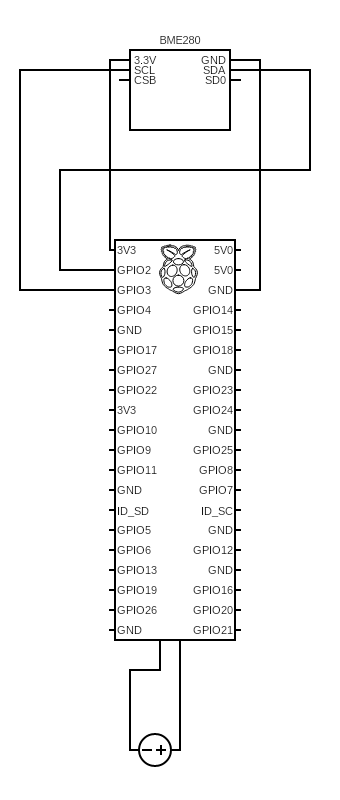
\includegraphics[width=.9\columnwidth]{figuras/circuit.png}
\caption{Esquemático de conexão do RPI3B com o sensor BME280}
\label{fig:exemplo_esquem}
\end{figure}

% A BOM tá basicamente feita se for só esse sensor até o final do projeto. 
\begin{table}[!htpb]
% increase table row spacing, adjust to taste
% \renewcommand{\arraystretch}{1.3}
\caption{Lista de materiais.}
\label{tab:BOM}
\centering
\begin{tabular}{ccc}
\hline
\textbf{Componente} & \textbf{Preço unitário} & \textbf{Quantidade}\\
\hline 
Módulo Sensor BME280 & R\$ 52,90 & 1 \\
Cabo Jumper Fêmea/Fêmea & R\$ 0,20 & 4 \\
\hline
\textbf{Total} & R\$ 53,70 & \\
\hline
\end{tabular}
\end{table}

Por fim, a Figura \ref{fig:diagramabloco} apresenta o diagrama de blocos do sistema, representando os principais componentes de hardware que serão utilizados para correto e completo funcionamento.

%had to do this atrocity with the height so it would fit 
\begin{figure}[!ht]
\centering
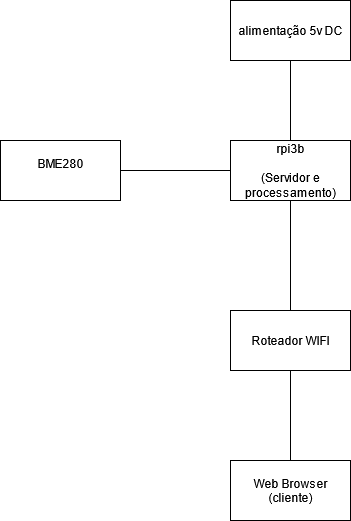
\includegraphics[width=.7\columnwidth]{figuras/diagramabloco.png}
\caption{Diagrama de blocos do sistema proposto}
\label{fig:diagramabloco}
\end{figure}

%Tópicos importantes a serem descritos nesta Subseção incluem:

%\begin{itemize}
%    \item \textbf{Processamento:} RPi 3, Arduino, MSP430 etc.
%    \item \textbf{Sensores:} tipos (temperatura, pressão etc.), taxas de amostragem e precisões necessárias;
%    \item \textbf{Atuadores:} motores DC, relés, LEDs etc.
%    \item \textbf{Comunicações:} UART, I2C, SPI, USB, WiFi, Bluetooth etc.
%    \item \textbf{Armazenamento:} \textit{hard drive}, cartão SD, \textit{pendrive} etc.
%    \item \textbf{Interfaces com o usuário:} botões, LEDs, display, touchscreen etc.	
%    \item \textbf{Estrutura física:} formato, dimensões, posicionamento dos circuitos, dos sensores, dos atuadores e da interface com o usuário.
%\end{itemize}
